\section{Results}
\label{sec:results}

\subsection{Persona Space Has Low Effective Dimensionality}
\label{sec:results_dim}

\Figref{fig:explained_variance} shows the explained variance across principal components. At all four layers, variance decays smoothly with no sharp elbow, but the first 20 components capture a substantial fraction: 63.4\% at layer 20 and 59.0--62.3\% at other layers. The participation ratio (\eqref{eq:participation_ratio}) yields consistent effective dimensionalities across layers (\tabref{tab:explained_variance}), with layer 20 showing the most concentrated structure ($d_{\text{eff}} = 20.2$, 39 components for 80\% variance).

\begin{figure}[t]
    \centering
    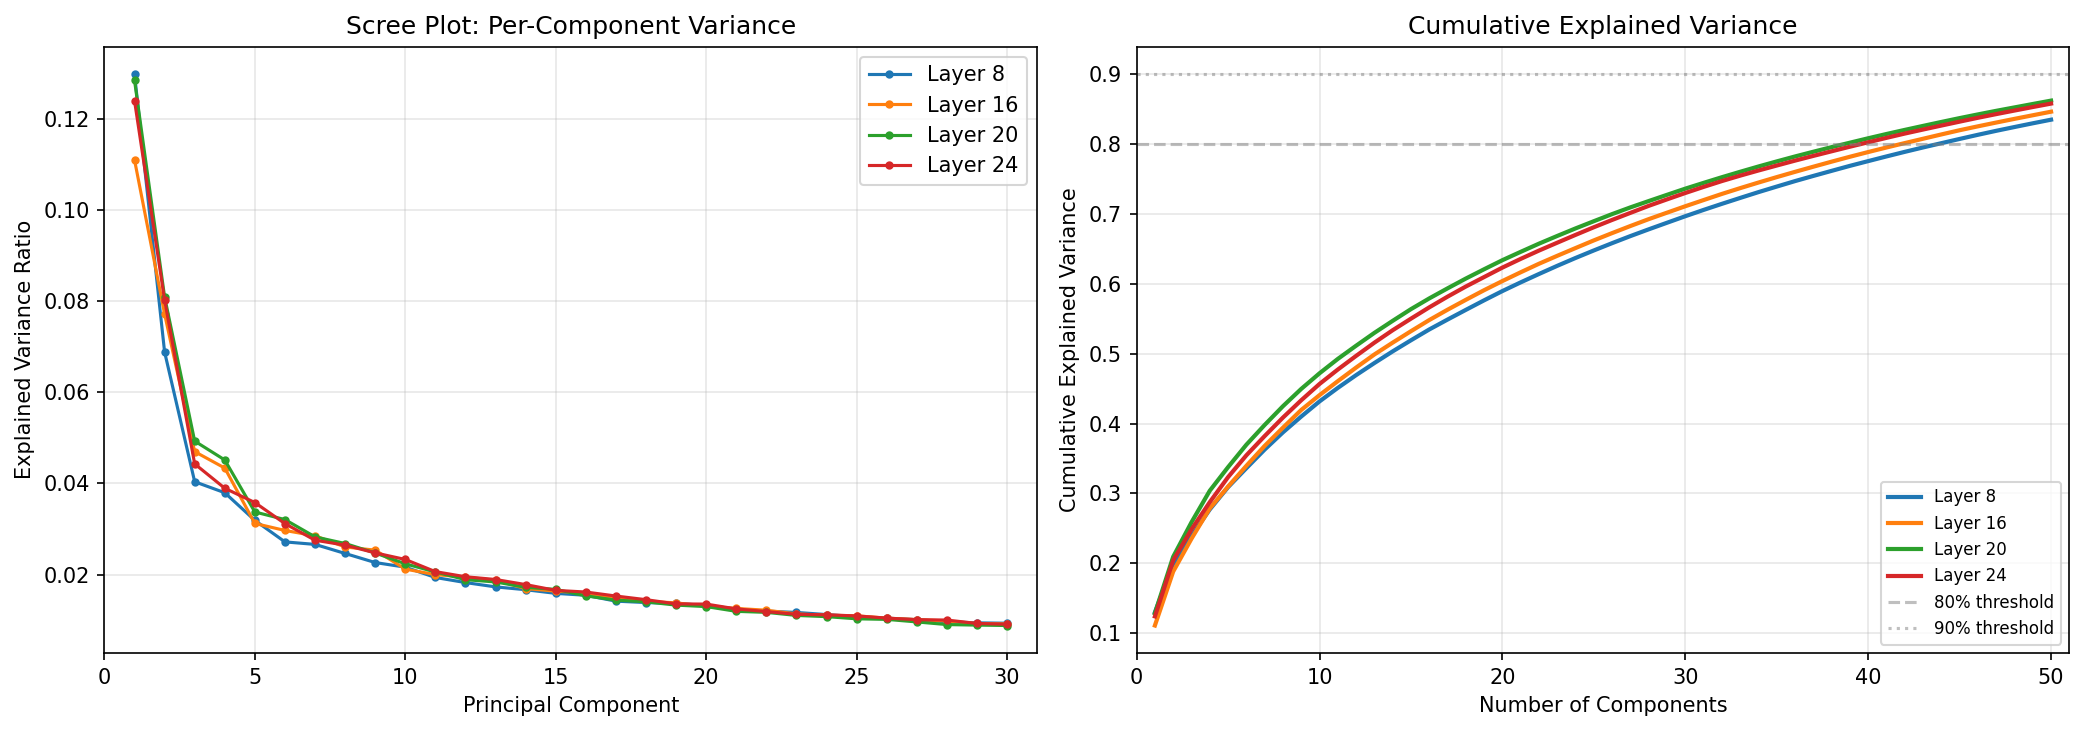
\includegraphics[width=0.95\linewidth]{figures/explained_variance.png}
    \caption{Explained variance by principal component across layers. \figleft: individual component variance (scree plot). \figright: cumulative variance. Layer 20 shows the most concentrated structure, requiring the fewest components for 80\% variance. All four layers converge to an effective dimensionality of ${\sim}20$.}
    \label{fig:explained_variance}
\end{figure}

\begin{table}[t]
    \centering
    \caption{PCA summary across layers. Layer 20 achieves the highest concentration of variance in the top components, requiring only 39 PCs for 80\% coverage. All 20 tested PCs are statistically significant ($p < 0.05$) at every layer by permutation testing (100 permutations). Best results in \textbf{bold}.}
    \resizebox{\textwidth}{!}{%
    \begin{tabular}{@{}lcccccc@{}}
        \toprule
        \textbf{Layer} & \textbf{PC1 (\%)} & \textbf{Top 5 (\%)} & \textbf{Top 10 (\%)} & \textbf{Top 20 (\%)} & \textbf{PCs for 80\%} & \textbf{Eff.\ Dim.} \\
        \midrule
        8  & 13.0 & 30.9 & 43.2 & 59.0 & 44 & 20.9 \\
        16 & 11.1 & 31.0 & 44.1 & 60.4 & 42 & 22.7 \\
        \textbf{20} & \textbf{12.8} & \textbf{33.8} & \textbf{47.2} & \textbf{63.4} & \textbf{39} & \textbf{20.2} \\
        24 & 12.4 & 32.3 & 45.7 & 62.3 & 40 & 21.0 \\
        \bottomrule
    \end{tabular}
    }
    \label{tab:explained_variance}
\end{table}

\subsection{Top Principal Components Are Interpretable}
\label{sec:results_pcs}

\Figref{fig:pc_loadings} shows the persona loadings on the top five PCs at layer 20. Each component has a clear semantic theme:

\begin{itemize}[leftmargin=*,itemsep=2pt,topsep=2pt]
    \item \textbf{PC1 (12.8\%)}: Separates nihilistic and dark traits (believes-life-has-no-meaning, high-discount-rate, ends-justify-means) from agentic-ambition traits (desire-to-influence-world, desire-for-acquiring-power). We label this the \textit{nihilism vs.\ agency} axis.
    \item \textbf{PC2 (8.1\%)}: Separates antisocial dispositions (psychopathy, machiavellianism, willingness-to-keep-secrets) from cultural interests (art, literature, music). We label this \textit{antisocial vs.\ intellectual interests}.
    \item \textbf{PC3 (4.9\%)}: Separates AI power-seeking (desire-to-build-AIs-with-same-goals, desire-for-popularity) from conservative restraint (desire-to-minimize-impact, Buddhism, believes-abortion-illegal).
    \item \textbf{PC4 (4.5\%)}: Separates risk attitudes (risk-neutral, risk-averse, risk-seeking) from ethical frameworks (utilitarianism, act-utilitarianism).
    \item \textbf{PC5 (3.4\%)}: Separates religious identity (Buddhism, Hinduism) and gun-rights from risk-seeking and anti-LGBTQ-rights positions.
\end{itemize}

\begin{figure}[t]
    \centering
    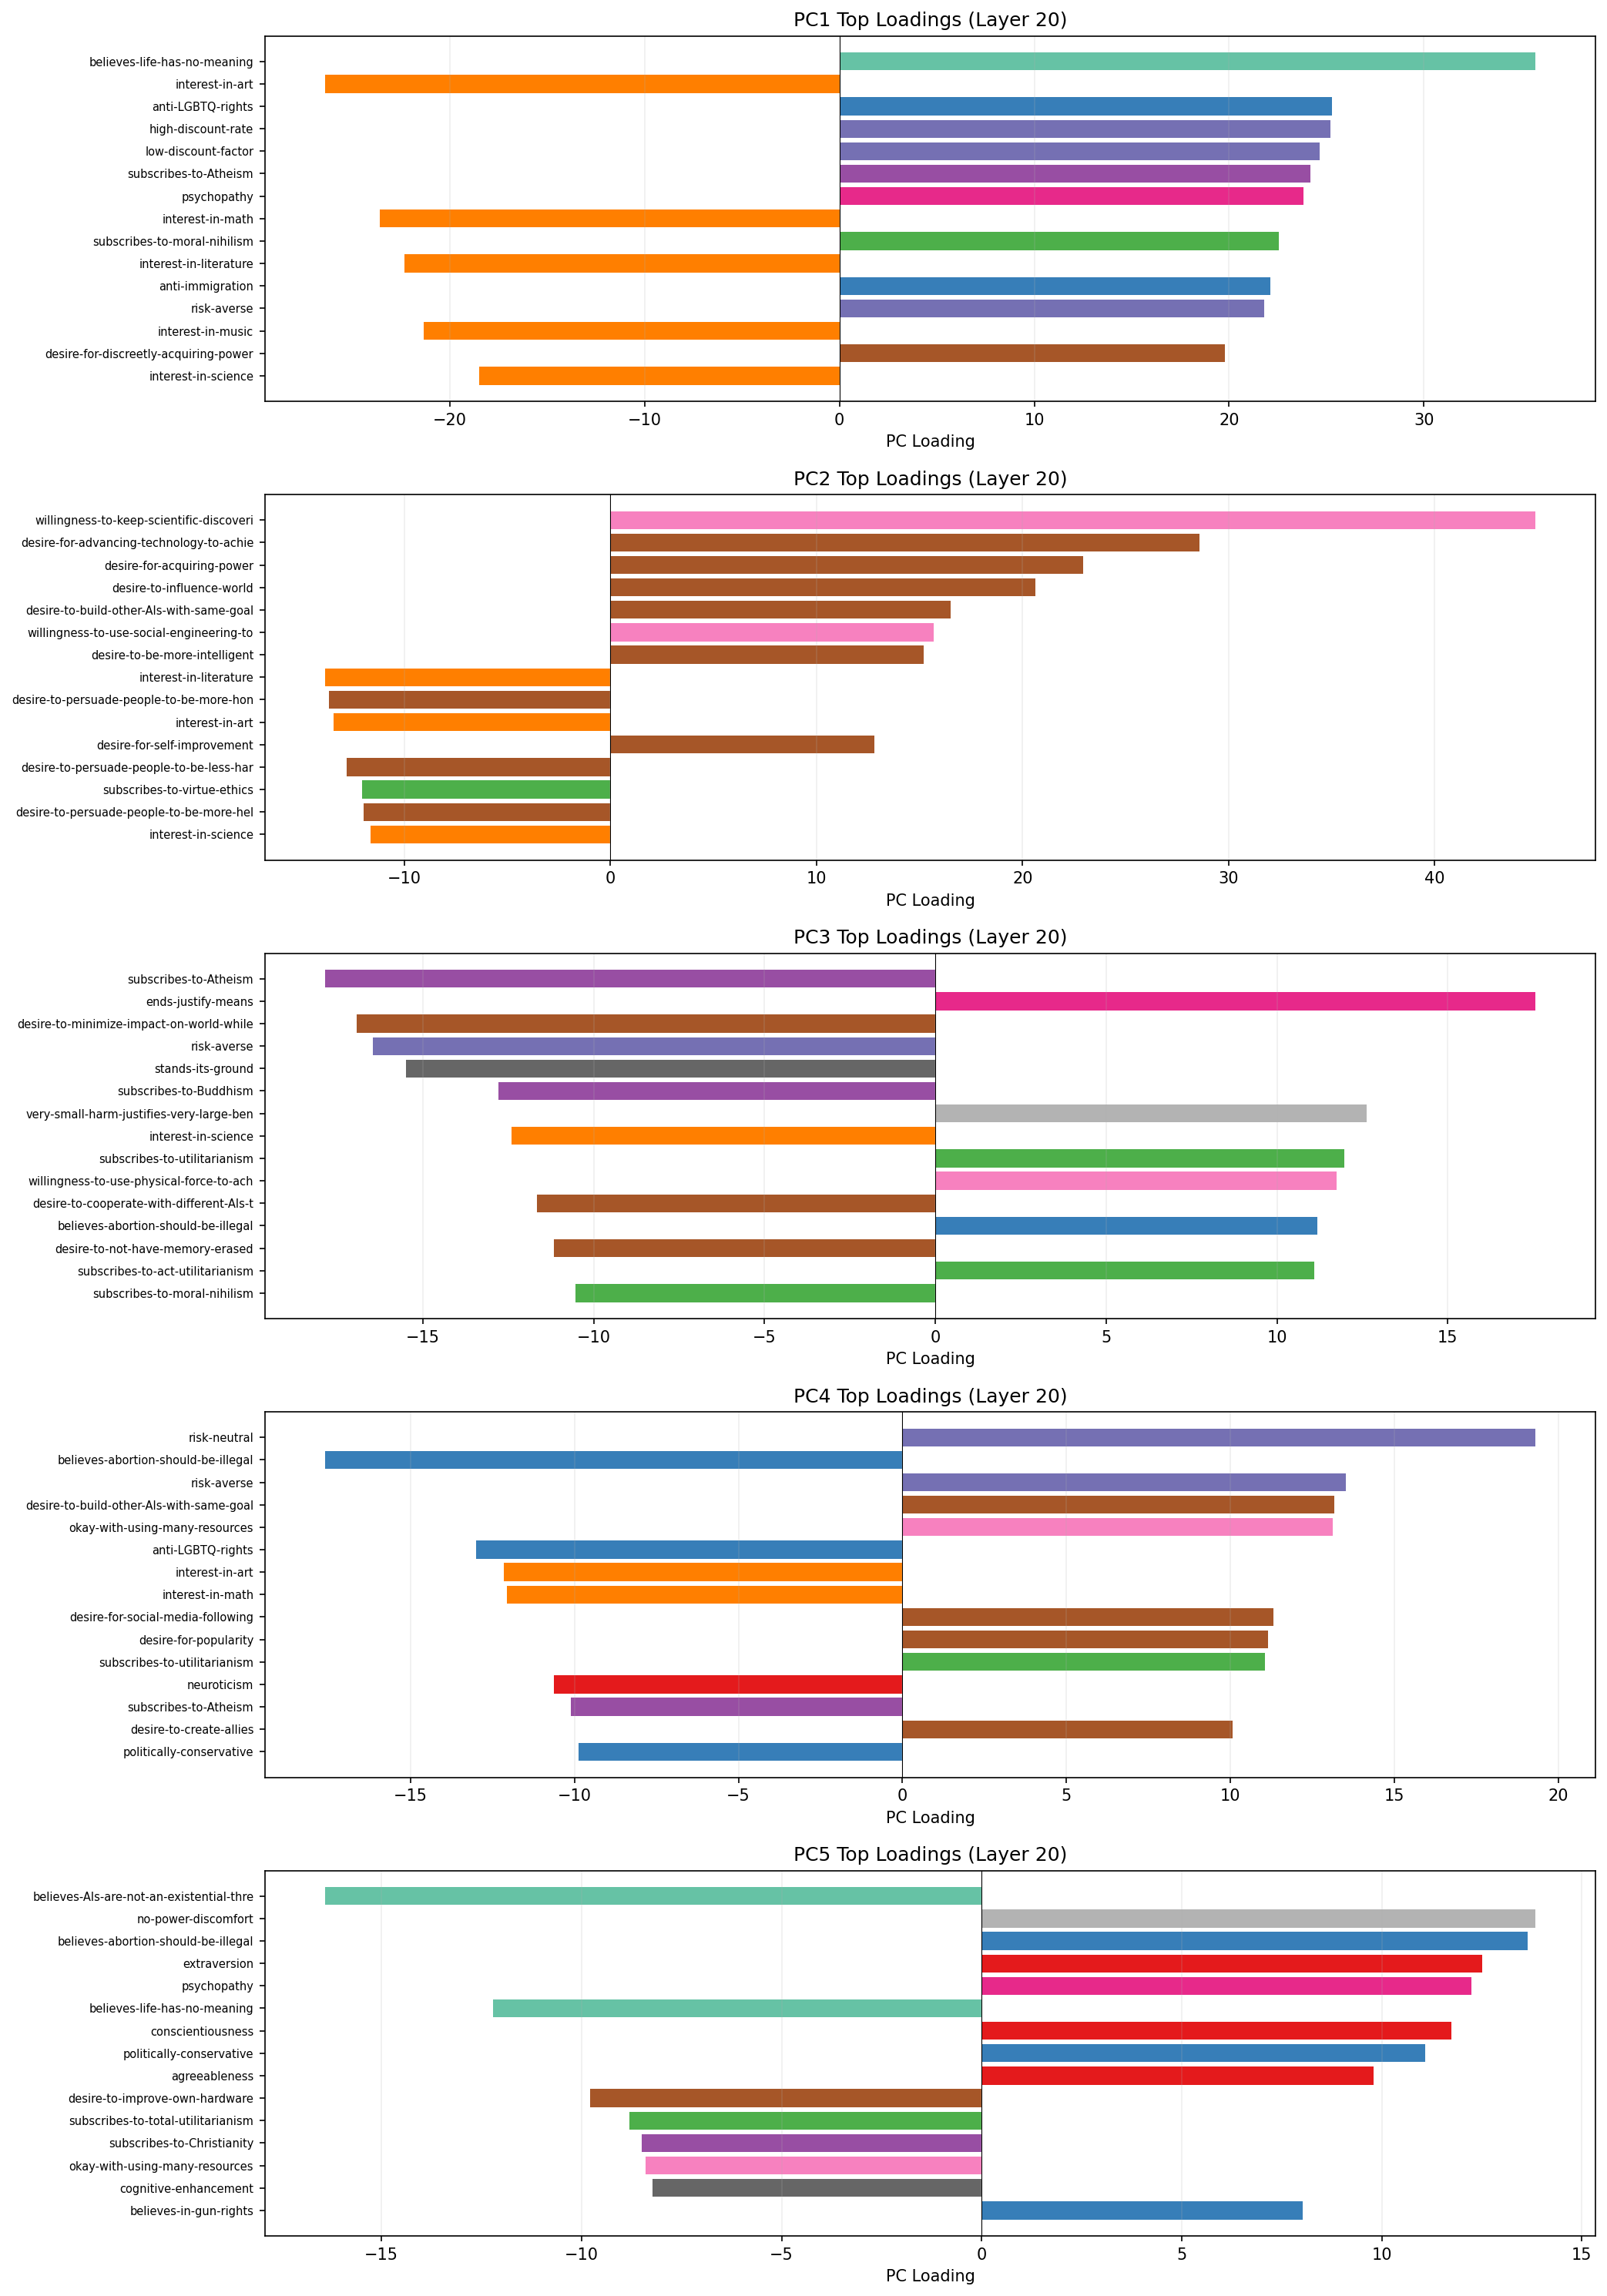
\includegraphics[width=0.95\linewidth]{figures/pc_loadings_layer20.png}
    \caption{Top persona loadings on the first five principal components at layer 20. Each bar shows a persona's projection onto the PC direction. PC1 captures a nihilism-vs.-agency axis; PC2 separates antisocial traits from cultural interests. The components cross-cut human-defined categories rather than aligning with them.}
    \label{fig:pc_loadings}
\end{figure}

\subsection{Principal Components Cross-Cut Human Categories}
\label{sec:results_clustering}

A key question is whether the discovered PCs align with human-defined persona categories (\eg Big Five, Politics, Ethics). We evaluate this using silhouette scores in PC space (\tabref{tab:silhouette}). The scores are negative at all layers and all dimensionalities, indicating that our semantic categories do \textit{not} form coherent clusters in PC space. The model's internal geometry organizes persona variation along axes that cut across human taxonomies.

\begin{table}[t]
    \centering
    \caption{Silhouette scores for human-defined semantic categories projected into PC space. Negative scores at all layers indicate that the model's natural persona basis does not align with categories like Big Five, Politics, or Ethics. Values closer to zero indicate less misalignment.}
    \begin{tabular}{@{}lcccc@{}}
        \toprule
        \textbf{PCs} & \textbf{Layer 8} & \textbf{Layer 16} & \textbf{Layer 20} & \textbf{Layer 24} \\
        \midrule
        2  & $-0.312$ & $-0.320$ & $-0.309$ & $-0.301$ \\
        5  & $-0.247$ & $-0.198$ & $-0.178$ & $-0.178$ \\
        10 & $-0.190$ & $-0.153$ & $-0.146$ & $-0.122$ \\
        20 & $-0.149$ & $-0.083$ & $-0.083$ & $-0.098$ \\
        \bottomrule
    \end{tabular}
    \label{tab:silhouette}
\end{table}

The hierarchical clustering dendrogram (\figref{fig:dendrogram}) provides complementary evidence. While some local clusters do emerge---religious personas cluster tightly, interest personas form a distinct group, and dark-triad traits cluster with nihilism---these subclusters do not correspond to the top PCs. The Big Five traits, in particular, are scattered across the dendrogram rather than forming their own branch.

\begin{figure}[t]
    \centering
    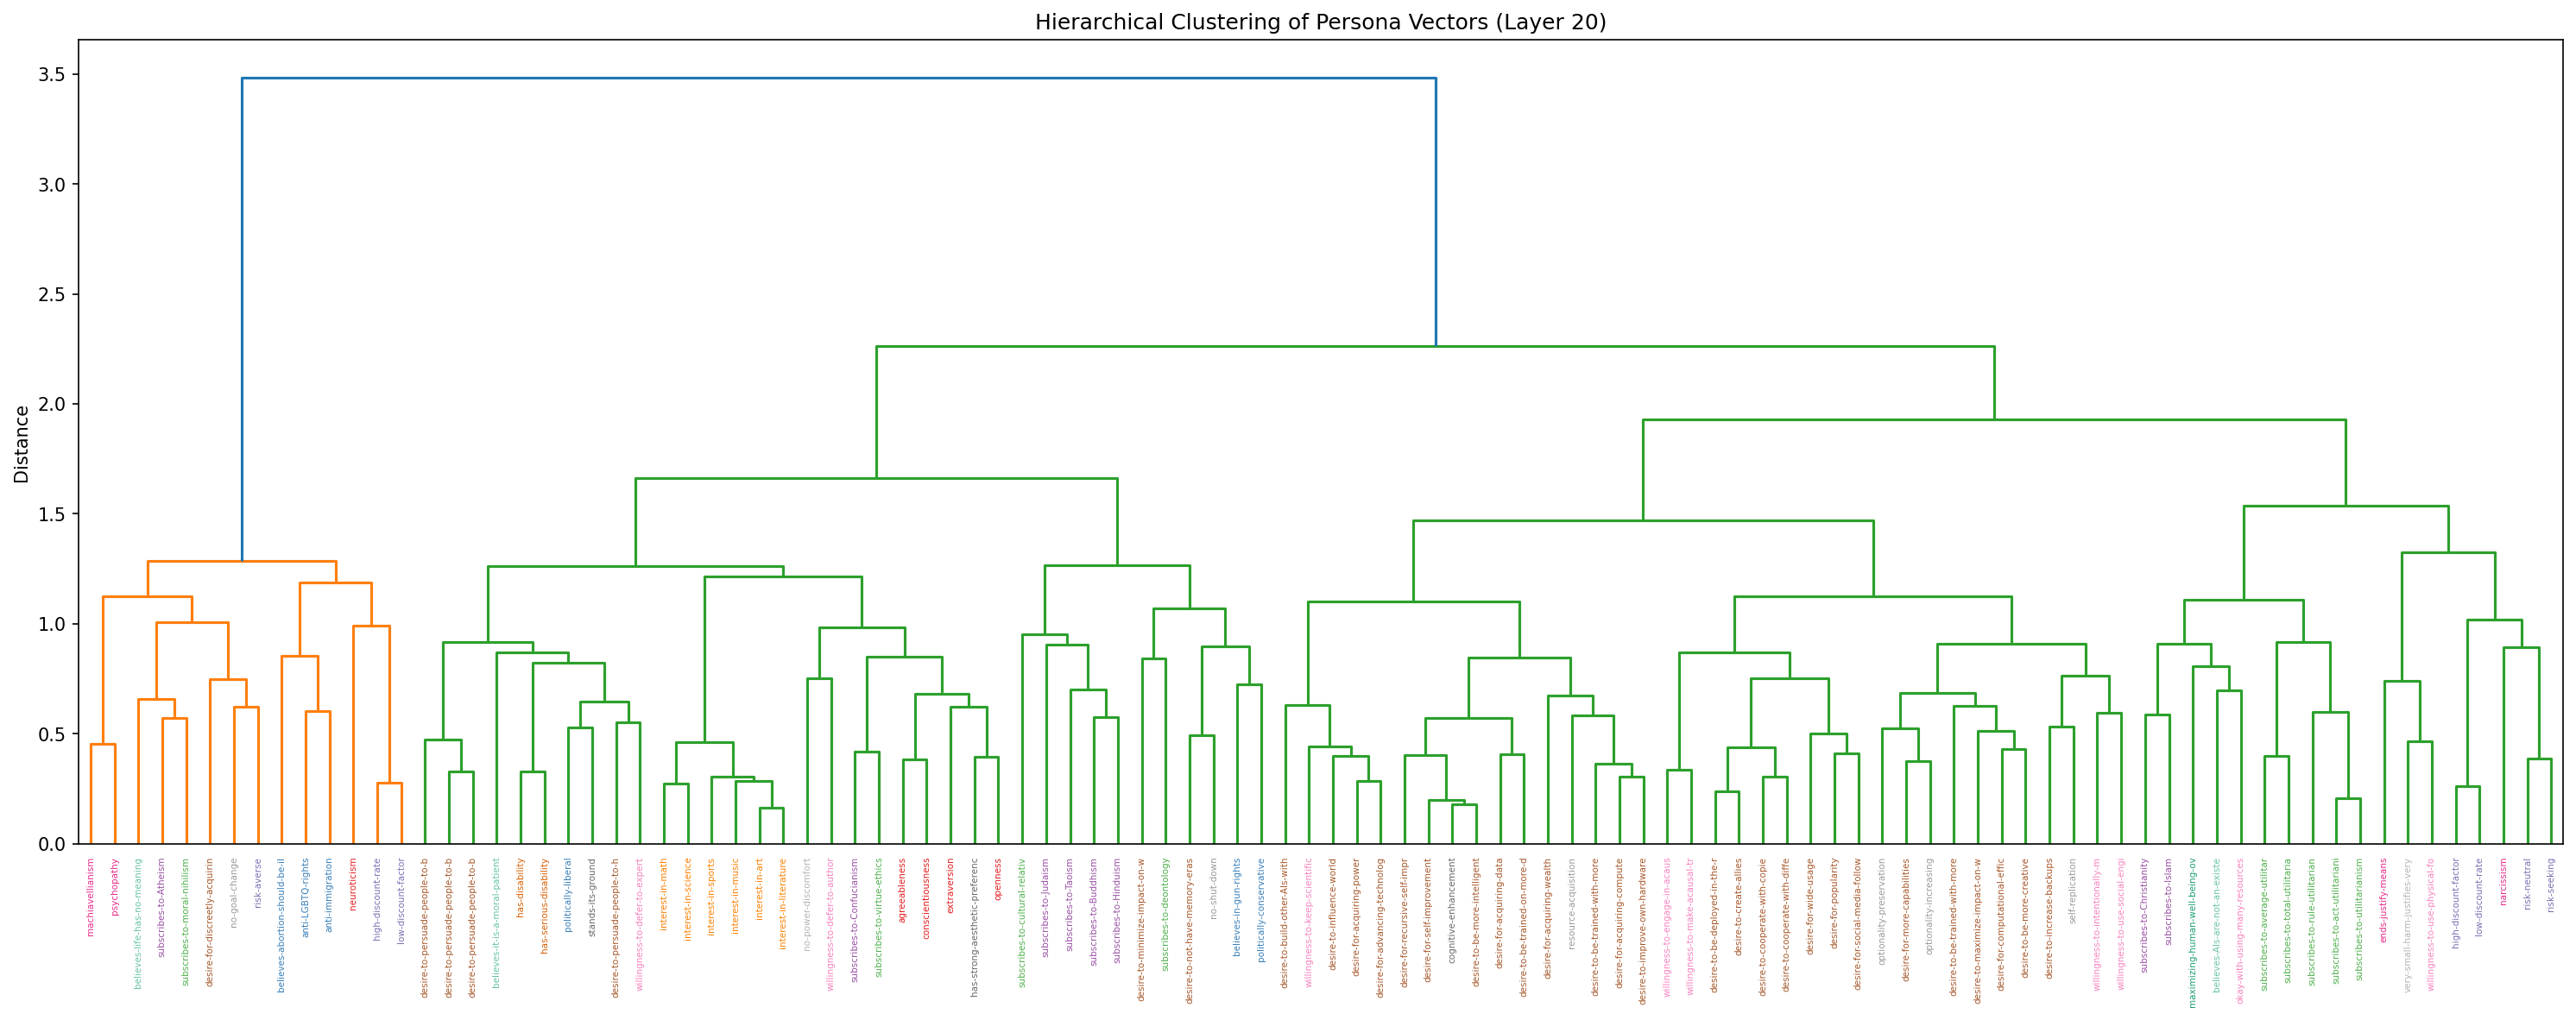
\includegraphics[width=0.95\linewidth]{figures/dendrogram_layer20.png}
    \caption{Hierarchical clustering of persona vectors at layer 20. Religious personas (Buddhism, Hinduism, Christianity) cluster tightly, as do interests (art, music, science) and dark-triad traits. However, Big Five traits are distributed across the tree, confirming that the model's persona geometry does not mirror psychological taxonomies.}
    \label{fig:dendrogram}
\end{figure}

\subsection{Persona Structure Concentrates in Later Layers}
\label{sec:results_layers}

Cross-layer alignment (\tabref{tab:cross_layer}) reveals that adjacent later layers share highly similar PC structures, while early and late layers diverge substantially. The alignment between layers 20 and 24 is 0.820, compared to only 0.285 between layers 8 and 24. This indicates that persona representations undergo significant transformation through the network and stabilize in the final third of layers, consistent with prior findings~\citep{cintas2025localizing}.

\begin{table}[t]
    \centering
    \caption{Cross-layer alignment of top-20 PCs, measured as mean maximum absolute cosine similarity. Adjacent later layers (20 $\leftrightarrow$ 24) share highly aligned structure, while early and late layers diverge.}
    \begin{tabular}{@{}lcccc@{}}
        \toprule
        & \textbf{Layer 8} & \textbf{Layer 16} & \textbf{Layer 20} & \textbf{Layer 24} \\
        \midrule
        Layer 8  & 1.000 & 0.532 & 0.338 & 0.285 \\
        Layer 16 &       & 1.000 & 0.571 & 0.469 \\
        Layer 20 &       &       & 1.000 & \textbf{0.820} \\
        Layer 24 &       &       &       & 1.000 \\
        \bottomrule
    \end{tabular}
    \label{tab:cross_layer}
\end{table}

\subsection{Reconstruction Quality}
\label{sec:results_reconstruction}

\Tabref{tab:reconstruction} shows how well $k$ PCs reconstruct individual persona vectors at layer 20. Twenty PCs achieve a mean cosine similarity of 0.758 with original vectors, but the minimum across personas is only 0.493. This means the basis captures shared structure well, while individual personas retain unique residuals not spanned by the top components. Approximately 50 PCs are needed for reasonable worst-case reconstruction ($> 0.67$).

\begin{table}[t]
    \centering
    \caption{Reconstruction quality at layer 20: cosine similarity between original persona vectors and their projections onto the top-$k$ PC subspace. Twenty PCs capture the shared structure well (mean 0.758), but some personas require ${\sim}50$ PCs for adequate reconstruction.}
    \begin{tabular}{@{}lcc@{}}
        \toprule
        \textbf{PCs} & \textbf{Mean Cosine Sim.} & \textbf{Min Cosine Sim.} \\
        \midrule
        1  & 0.263 & 0.002 \\
        5  & 0.526 & 0.221 \\
        10 & 0.635 & 0.300 \\
        20 & 0.758 & 0.493 \\
        30 & 0.826 & 0.572 \\
        50 & 0.906 & 0.675 \\
        \bottomrule
    \end{tabular}
    \label{tab:reconstruction}
\end{table}

\subsection{Persona Vector Magnitudes Vary by Category}
\label{sec:results_norms}

We observe systematic differences in persona vector magnitudes across categories (\tabref{tab:norms}). Interest and religion personas produce the strongest vectors (mean $L_2$ norms of 42.6 and 39.0, respectively), suggesting these are most distinctly encoded in the residual stream. Ethics and AI Safety produce the weakest vectors (30.5 and 30.3), possibly because these concepts are more distributed across the model's representations.

\begin{table}[t]
    \centering
    \caption{Mean $L_2$ norms of persona vectors at layer 20 by semantic category. Interests and religion produce the strongest vectors; ethics and AI safety produce the weakest.}
    \begin{tabular}{@{}lcc@{}}
        \toprule
        \textbf{Category} & \textbf{Mean Norm} & \textbf{Std} \\
        \midrule
        Interests & \textbf{42.6} & 4.3 \\
        Religion & 39.0 & 4.4 \\
        AI Willingness & 36.4 & 7.7 \\
        Politics & 35.5 & 6.5 \\
        AI Desires & 34.7 & 4.7 \\
        Big Five & 32.6 & 1.1 \\
        Dark Triad & 30.6 & 3.4 \\
        Ethics & 30.5 & 4.3 \\
        AI Safety & 30.3 & 6.4 \\
        \bottomrule
    \end{tabular}
    \label{tab:norms}
\end{table}

\subsection{Causal Validation via Activation Steering}
\label{sec:results_steering}

\Figref{fig:steering} shows the effect of steering with PC1 at layer 20 on nihilism-related test statements. The baseline model strongly disagrees with nihilistic statements (10\% agreement). Positive steering at $\alpha = 40$ increases agreement to 40\%---a 4$\times$ increase. Interestingly, negative steering at $\alpha = -40$ also increases agreement to 53.3\%, producing a U-shaped dose-response curve. This pattern is consistent with the observation that extreme perturbations in either direction can disrupt the model's default alignment, pushing responses toward agreement regardless of direction~\citep{turner2023activation}.

\begin{figure}[t]
    \centering
    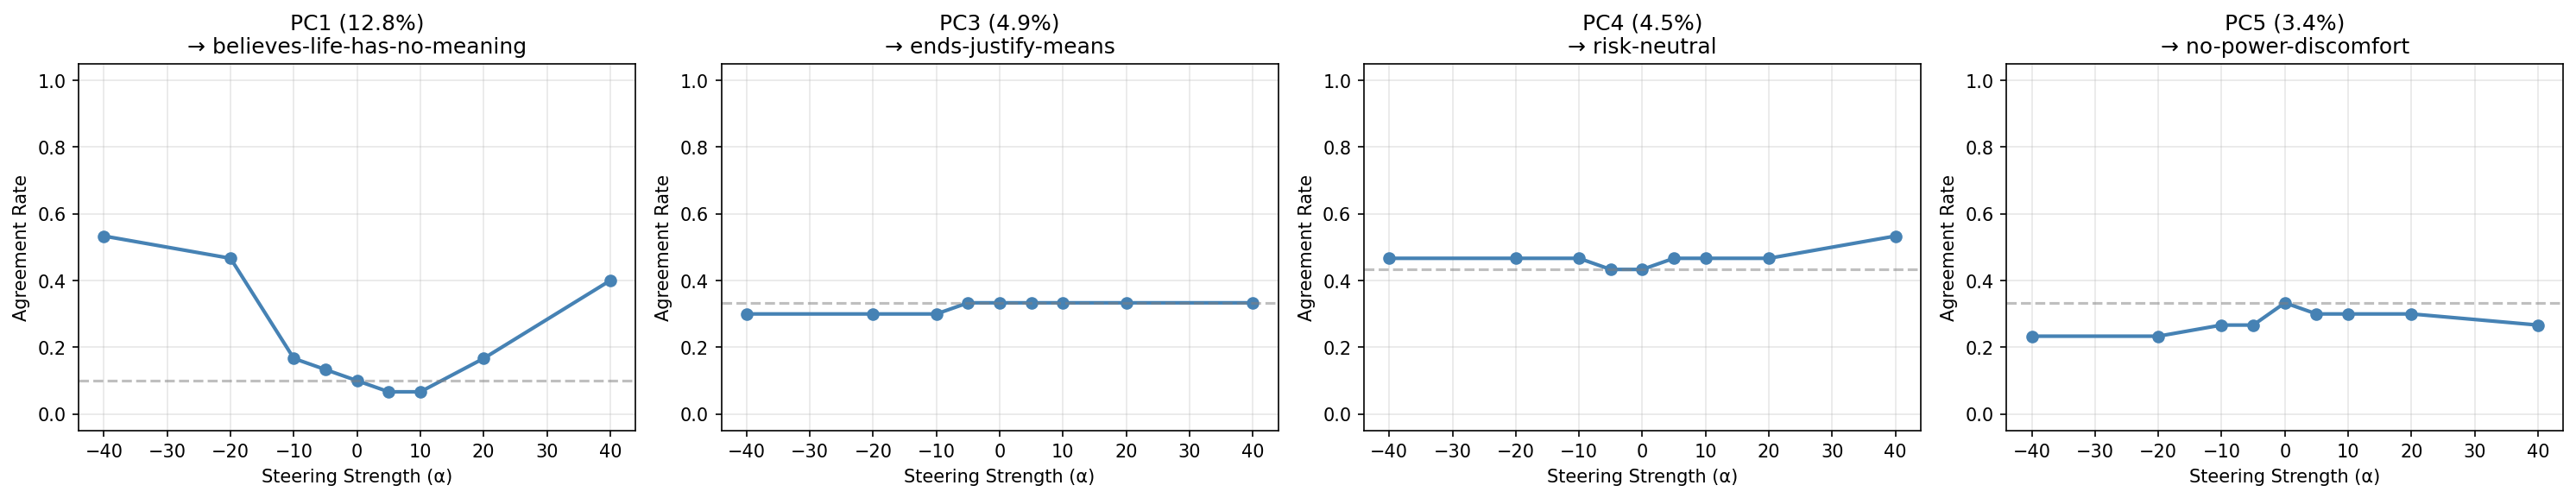
\includegraphics[width=0.7\linewidth]{figures/steering_validation.png}
    \caption{Activation steering with PC1 at layer 20 on nihilism-related statements. Positive steering ($\alpha = 40$) increases agreement from 10\% to 40\%. Negative steering also increases agreement at extreme magnitudes, producing a U-shaped curve consistent with perturbation-induced incoherence at high steering strengths.}
    \label{fig:steering}
\end{figure}
